%%
%% VERSION HISTORY
%%    22 May 2006 - John Papandriopoulos - Original version
%%    12 Jul 2007 - John Papandriopoulos - Converted into template
%%

\chapter{Tools and resources}
	\label{chapter:empire-strikes-back}%
	%

% preferred location for figures in this chapter
\setfigurepath{figures/chapter-3}

%=========================================================================

%=========================================================================
\section{Framework and libraries}
\subsection*{NLTK}
NLTK\footnote{http://www.nltk.org/} (\textbf{N}atural \textbf{L}anguage \textbf{T}ool\textbf{K}it) is a popular framework for working with human language. It is developed by Steven Bird\footnote{http://www.stevenbird.net/}, Ewan Klein\footnote{http://homepages.inf.ed.ac.uk/ewan/} and Edward Loper\footnote{http://ed.loper.org/}. The project was started in 2001 and still continue to update and release at the time of writing. The platform provides a suite of processing libraries for text classification, stemming, tokenization, parsing, tagging and semantic reasoning functionalities. It also serve as wrappers for other NLP libraries such as Stanford CoreNLP \cite{manning-EtAl:2014:P14-5}. We can easily access more than 50 corpora and other lexical resources such as WordNet\textsuperscript{\textregistered} through interfaces of Python programming language.\\
Authors of NLTK also published the book \textit{Natural Language Processing with Python} \cite{Bird2009} to give practical introduction and hands-on guide to programming for NLP. The book covers many topics of computational linguistic, their examples by graphical demonstrations and sample data. Along with comprehensive online documentation, readers learn the fundamentals of writing Python scripts for NLP tasks like categorizing text, working with corpora and analyzing linguistic structure of them. Both NLTK and the book are free of charge and publicly available online. As a result, NLTK is used as a teaching tool for NLP education in many universities around the world.\\

\subsection*{Scikit-learn}
Scikit-learn\footnote{http://scikit-learn.org/} is a free software package for machine learning and data analysis written in Python \cite{scikit-learn}. The project was originally started in 2007 by David Cournapeau\footnote{https://github.com/cournape} and still under active development as of 2017 by many different researchers and developers. Like NLTK, scikit-learn is designed for Python and compatible with other numerical and scientific Python libraries like NumPy and SciPy. Scikit-learn features machine learning algorithms for classification, clustering and regression tasks such as linear regression, SVM, k-means, decision tree and boosting. It is very well-maintained with stable release and online documentation on its website. Furthermore, each algorithm and its variant are illustrated by practical examples including brief explanation with citation, figures and sample code with comments to enhance readers' understanding of the problem. 


\section{Employed NLP methods}
\subsection*{Tokenization}
\textit{Tokenization} is usually a crucial step appearing in early stage of the NLP workflow to facilitate processing with more complex analytical techniques. Tokenization is the task of divide a character sequence into defined document units referred as tokens. A token is defined as "an instance of a sequence of characters in some particular document that are grouped together as a useful semantic unit for processing" \cite{Manning:2008:IIR:1394399}. In theory, tokens can take form of any textual elements of chosen granularity such as punctuation or fomulae but in practice, tokens are usually words.\\

\begin{figure}
\centering
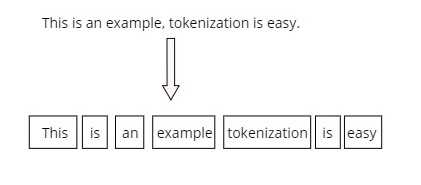
\includegraphics[width=\textwidth, clip=true, height = 5.5cm]{img/tokenization_example}
\caption[Tokenization example]{ Example of tokenization. Tokenizer splits a sentence into words.} 
\label{fig:token_ex1}
\end{figure}

As shown in Figure~\ref{fig:token_ex1}, tokenization have dropped punctuation of the sentence and each word is getting full meaning. However, tokenization phase may encounters difficult choice in a broader context. For example, take a look at the sentence "\textit{Tokenization isn't easy}". Two words \framebox{Tokenization} and \framebox{easy} are pretty straightforward since they are splitted by whitespace. In contrast, \textit{isn't} can be tokenized by different rules: \framebox{isn't}, \framebox{isnt}, \framebox{is} \framebox{n't}, \framebox{isn} \framebox{t}. Furthermore, each language and topic contain jargon and words refer to specific entities but are not in standard dictionary. For instance, AK-47 is name of a semi-automatic rifle, programming language C\# and so on. Computer era brings new types of technology terminology, which appear frequently on online document, such as website addresses (https://www.google.com/), email adresses (johndoe@gmail.com), decimal IP addresses (123.172.2.1). These character sequences should be recognize as one entity but in some cases, it would cause unnecessary index to be included in the extracted dictionary. In the experiment of this thesis, NLTK Tokenizer package, which is improved TreebankWordTokenizer \footnote{http://www.nltk.org/api/nltk.tokenize.html\#nltk.tokenize.treebank.TreebankWordTokenizer} along with PunktSentenceTokenizer\footnote{http://www.nltk.org/api/nltk.tokenize.html\#nltk.tokenize.punkt.PunktSentenceTokenizer} for the specified language, was used.\\

\subsection*{Stop words removal}
\textit{Stop words} are words that contribute very little in term of semantic, thus being considered low value in IR systems. These words usually appear with high frequency in collection. To remove stop words, high use words must be manually assessed for semantic content. If a word is identify as a stop word, it is added to a list called \textit{stop list}. The length of a stop list varies between less than twenty (15-18 terms) to a few hundred words (200-300 terms). Depeding on purpose and scale of a system, a stop list can be very general or specifically relate to a topic.\\
Using a stop list can potentially reduce query time due to smaller index of a system. However, web search engines in practice do not use stop lists partially because of immense server clusters behind them generating enormous computing power. \\
Common words belong to world classes article, conjunction, preposition and frequent words like \textit{now} or \textit{very} are included in stop lists. General-purpose stop lists are available online and can be easily incorporated into IR systems. Sometimes removing stop words can be detrimental as vital information may be missed after going through stop list filter (e.g. \textit{"To be or not to be"} is a well known verse that may get taken out of indexed vocabulary) so utilization of these lists must be carefully examined. In the experiment of this thesis, Stopwords corpus of NLTK was used. It is a corpus containing 2400 stopwords for 11 languages. Stop list for English contain 153 words.\\

\subsection*{Part-of-speech tagging}
A Part-of-speech (POS) tag is category of words assigned to a word which display similar (primarily syntactic) grammatical properties of it in the sentence. Words that share the same POS tag 
typically play similar roles in structure of sentences. Example of some POS tags are NOUN (noun), ADJ (adjective), VERB (verb), PRON (pronoun). In practice, there are many sets of POS tag (tagset) such as Universal\footnote{http://universaldependencies.org/u/pos/}, Treebank. Some tagsets usually comprise fine-grained tag like "singular proper noun" for more complex analyzing task. In early years of building automatic POS tagger, handwritten rules distinguish parts of speech much like decision tree. These rules may work in a particular type of document or some set of rules can be applied widely to many text corpora of a language.\\
When machine learning techniques are utilized for POS tagging task, there are three main approaches: statistical tagging, rule-based tagging and hybrid tagging. Statistical tagging relied on corpora annotated by human as training data to compute probability of a specific token belong to a POS tag category. The drawback of statistical tagger is some tagged sequences are not correct due to low usage in a language. In other word, it is susceptible to rare case of word in an unfamiliar context and most of the time misclassify to usual tag of that word. Hybrid approach require both hand coded rules and probabilistic features of words, but it is not widely used in practice since balancing weight between these two features is not an easy task for a general-purpose tagger.\\
\begin{figure}
\centering
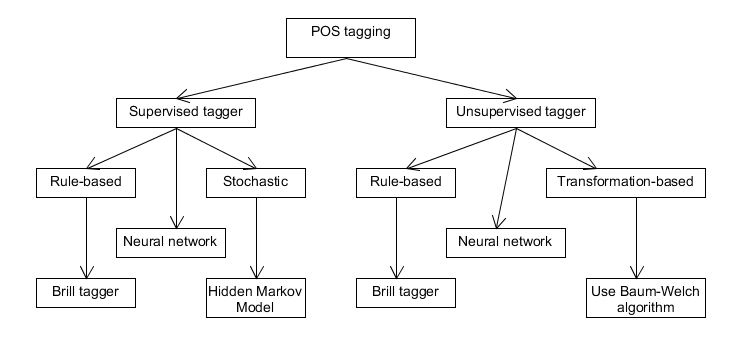
\includegraphics[width=\textwidth, clip=true]{img/POS_tagger}
\caption[POS tagger classification]{POS tagger classification} 
\label{fig:pos_tag}
\end{figure}
Figure~\ref{fig:pos_tag} shows classification of POS tagger. Neural network, rule-based tagger can be either supervised or unsupervised learning paradigm. Popular tagger are going to be introduced below.\\
\textbf{Unigram tagger:} Unigram tagger is the simplest tagger. It is a classifier trained on an annotated corpus, computing probability of of a tag assigned for a word and save it to a probability table or dictionary. When assigning POS tag for a particular word, it look up the table and choose the most probable tag (tag with highest probability) for that word. The default tag for unseen words in training data is NOUN. Unigram tagger is fast and may achieve high accuracy given the training corpus is huge enough. Furthurmore, unigram tagger can serve as baseline for more advanced tagger as it is very easy to build. \\
\textbf{Transformation-based tagger:} The output of unigram tagger become input of transformation-based tagger to produce rules of tagging sequentially. These rules are assessed based on improved accuracy compared to accuracy of unigram tagger. Rules that improves accuracy the most or more than a established threshold are going to be added to set of rules of other taggers or as standalone tagging system.\\
\textbf{Hidden Markow Model (HMM):} HMM based tagger is also a statistical tagger, finding the most likely tag for words in sentence. Unlike unigram tagger, which tag each word separately, HMM tagger assigns a sequence of tag to sequence of word in sentences. The underlying idea is for a sequence of words, what is the most probable sequence of tag for that. Given a sentence \textit{w\textsubscript{1}, w\textsubscript{2}, ... , w\textsubscript{n}}, a tag sequence \textit{t\textsubscript{1}, t\textsubscript{2},..., t\textsubscript{n}} is assigned to the sentence if it produce the maximum the joint probability:
\begin{eqnarray*}
P(t\textsubscript{1}t\textsubscript{2}...\textsubscript{n} , w\textsubscript{1}w\textsubscript{2}...w\textsubscript{n}) = P(t\textsubscript{1}, t\textsubscript{2},..., t\textsubscript{n}) P(w\textsubscript{1}, w\textsubscript{2},..., w\textsubscript{n})
\end{eqnarray*}
It is not a good practice to compute \textit{P(t\textsubscript{1}, t\textsubscript{2},..., t\textsubscript{n})} directly as the sentence may be quite long and computation become expensive. To cope with the problem, Markov assumption was proposed to simplify the equation. First-order Markov assumption states that the probability of a state depends only on the previous state, meaning the tag of a word is related only to the tag of previous word and not other words in the sentence.
\begin{eqnarray*}
P(t\textsubscript{i} \vert t\textsubscript{1}t\textsubscript{2}...\textsubscript{i-1}) = P(t\textsubscript{i} \vert t\textsubscript{i-1})
\end{eqnarray*}
\textbf{Maximum Entropy (ME) based tagger:} Both the introduced probabilistic models namely unigram and HMM tagger are simple and easy to build. However, due to structure of the models, adding more features to those models is challenging. Fortunately, the ME based tagger provide a way to easily incorporate more complex features into probability-based model \cite{Ratnaparkhi1996}. Given a sentence\textit{w\textsubscript{1}, w\textsubscript{2},..., w\textsubscript{n}}, ME model approximate the conditional probability of sequence \textit{t\textsubscript{1}, t\textsubscript{2},..., t\textsubscript{n}}
\begin{eqnarray*}
P(w_{1}, w_{2},..., w_{n} \vert t_{1}, t_{2},..., t_{n}) \approx \prod_{i=1}^{N} P(t_{i} \vert C_{i})
\end{eqnarray*}
where \textit{C\textsubscript{1}, C\textsubscript{2},..., C\textsubscript{n}} correspond to context of words in the sentence. A word \textit{w} have the context \textit{C} which is previous tags of words before \textit{w}. ME model present the idea of context that help predicting the tag of a word, which sounds very intuitive and logical. Context in this case is binary functions. The ME based tagger uses the context features to calculate conditional probability \textit{P(t\textsubscript{i} $\vert$ C\textsubscript{i})}. The weights of features are learned from training corpus to maximize the entropy of the model.\\
POS tagging plays an important role in the experiment of this thesis as we need to extract tags like nouns, verbs, adverbs. We used NLTK tagger, a neural network tagger trained on Penn TreeBank corpus.
\subsection*{Sentiment analysis}




